\documentclass[a4paper, 11pt]{article}
\usepackage[T1]{fontenc}
\usepackage{lmodern}
\usepackage[utf8]{inputenc}
\usepackage{tikz}
\title{Implementing Bentley Ottmann}
\begin{document}
\maketitle
\section{Comparing paths}
\subsection{Segments}
\begin{figure}[htbp]
  \begin{center}
    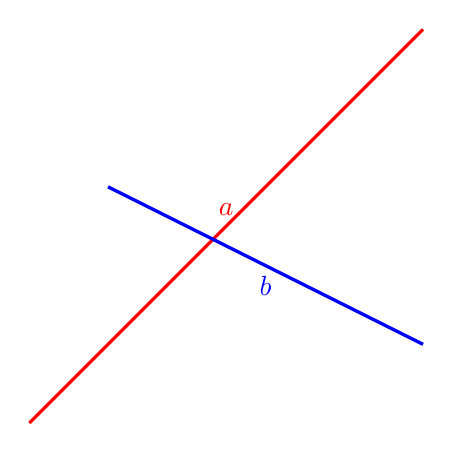
\begin{tikzpicture}
      \draw[very thick, draw=red] (0,0) edge node[above,text=red] {$a$} (5,5);
      \draw[very thick, draw=blue] (1,3) edge node[below,text=blue] {$b$} (5,1);
    \end{tikzpicture}
  \end{center}
  \caption{Is $a$ above $b$ ?}
  \label{fig:above}
\end{figure}

We maintain a set of alive paths during the whole algorithm.
This set requires to be sorted from topmost to bottom most.
An important question is therefore how to compare two different segments in order to
figure out which one is the topmost one.
We can see on Figure~\ref{fig:above} that most paths are not directly comparable.
Here we can see that on the left side $b$ is above $a$ while on the right side
$b$ is below $a$. Therefore which segment is the topmost one ?

The question as such is meaningless. In fact we need to add one more input and rephrase our
comparison question as : being given $a$, $b$ and a current position point $p$, which segment is
the topmost segment ?

\begin{figure}[htbp]
  \begin{center}
    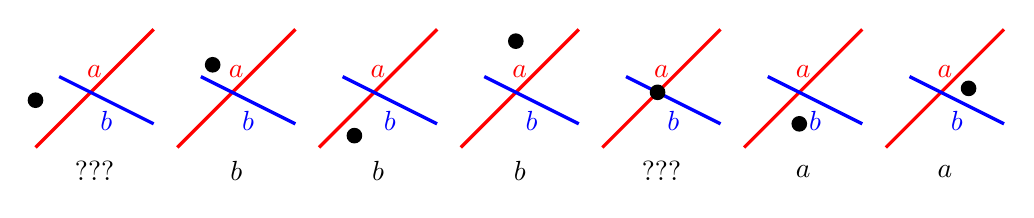
\begin{tikzpicture}[scale=0.3]
      \draw[very thick, draw=red] (0,0) edge node[above,text=red] {$a$} (5,5);
      \draw[very thick, draw=blue] (1,3) edge node[below,text=blue] {$b$} (5,1);
      \node[circle, fill=black, inner sep=2pt] at (0,2) {};
      \node at (2.5,-1) {???};
      \begin{scope}[xshift=6cm]
        \draw[very thick, draw=red] (0,0) edge node[above,text=red] {$a$} (5,5);
        \draw[very thick, draw=blue] (1,3) edge node[below,text=blue] {$b$} (5,1);
        \node[circle, fill=black, inner sep=2pt] at (1.5,3.5) {};
        \node at (2.5,-1) {$b$};
      \end{scope}
      \begin{scope}[xshift=12cm]
        \draw[very thick, draw=red] (0,0) edge node[above,text=red] {$a$} (5,5);
        \draw[very thick, draw=blue] (1,3) edge node[below,text=blue] {$b$} (5,1);
        \node[circle, fill=black, inner sep=2pt] at (1.5,0.5) {};
        \node at (2.5,-1) {$b$};
      \end{scope}
      \begin{scope}[xshift=18cm]
        \draw[very thick, draw=red] (0,0) edge node[above,text=red] {$a$} (5,5);
        \draw[very thick, draw=blue] (1,3) edge node[below,text=blue] {$b$} (5,1);
        \node[circle, fill=black, inner sep=2pt] at (2.333333,4.5) {};
        \node at (2.5,-1) {$b$};
      \end{scope}
      \begin{scope}[xshift=24cm]
        \draw[very thick, draw=red] (0,0) edge node[above,text=red] {$a$} (5,5);
        \draw[very thick, draw=blue] (1,3) edge node[below,text=blue] {$b$} (5,1);
        \node[circle, fill=black, inner sep=2pt] at (2.333333,2.333333) {};
        \node at (2.5,-1) {$???$};
      \end{scope}
      \begin{scope}[xshift=30cm]
        \draw[very thick, draw=red] (0,0) edge node[above,text=red] {$a$} (5,5);
        \draw[very thick, draw=blue] (1,3) edge node[below,text=blue] {$b$} (5,1);
        \node[circle, fill=black, inner sep=2pt] at (2.333333,1) {};
        \node at (2.5,-1) {$a$};
      \end{scope}
      \begin{scope}[xshift=36cm]
        \draw[very thick, draw=red] (0,0) edge node[above,text=red] {$a$} (5,5);
        \draw[very thick, draw=blue] (1,3) edge node[below,text=blue] {$b$} (5,1);
        \node[circle, fill=black, inner sep=2pt] at (3.5,2.5) {};
        \node at (2.5,-1) {$a$};
      \end{scope}
    \end{tikzpicture}
  \end{center}
  \caption{Which one is above ?}
  \label{fig:comparing}
\end{figure}

Fig.~\ref{fig:comparing} shows some expected answers for different positions.
Remark that it poses problem when the input position is exactly the intersection
of the two segments since the comparison becomes meaningless again.
To solve this problem we do the following~:
\begin{itemize}
  \item just before reaching the intersection, $b$ is above $a$ in our set.
  \item we the remove both segments.
  \item set the position to the intersection.
  \item re-inserts both segments with $a$ above $b$.
\end{itemize}

The meaning here is that being at the intersection is in fact being
right after meeting the intersection.

In order to ease the comparison process, we define a \emph{comparison_key} function
taking a segment, a position and returning a key. Comparing two segments will then
only require comparing their corresponding keys.


\end{document}
